\chapter{Results}

\section{Introduction}

As previously stated, this chapter describes the process of tuning the parameters of the genetic algorithm and the results obtained from the experiments.

\section{Iteration 1: Default Parameters}

This first iterations consists of the most basic configuration of the genetic algorithm with literature defaults \cite{literature-defaults}.

\begin{table}[h]
    \centering
    \begin{tabular}{|c c|}
        \hline
        \textbf{Parameter} & \textbf{Value} \\
        \hline
        POPULATION\_SIZE & 100 \\
        CXPB & 0.5 \\
        MUTPB & 0.2 \\
        K\_TOURNAMENT & 3 \\
        NUMBER\_OF\_GENERATIONS & 1 000 000 \\
        \hline
    \end{tabular}
    \caption{Parameters for Iteration 1}
    \label{tab:iteration1_parameters}
\end{table}

The currently implemented genetic algorithm struggles to find a valid solution for MPI and LPI instances. The evaluation limit makes the algorithm stop before a valid individual is found. The main reason could be the penalty value, which is set to the max weight of the vertices. This is a fixed value that doesn't scale well for higher problem sizes. This gives a hint that the penalty value should be set to a value that is proportional to the problem size. In particular, many different formulas have been used to calculate the penalty value, but none of these have shown any improvement.

The chosen solution is to remove the penalty mechanism and replace it with a repair mechanism that will fix the invalid individuals. It will perform a greedy repair by selecting the vertex with best ratio of covered edges over total weight. This repair mechanism is not perfect, but it's a good compromise between efficiency and accuracy.
This ensures that the genetic algorithm will always return a valid solution, even if it's not the best one.

\begin{lstlisting}[caption=Repair mechanism]

function repair(individual):
    WHILE any edge (u,v) is not covered by individual:
        Find vertex w with lowest (weight/number_of_uncovered_edges_it_covers)
        individual[w] = 1
    RETURN individual
end
\end{lstlisting}

Since the algorithm was now very slow, a compromise was made: the repair mechanism was only applied for the first generation. This way, the genetic algorithm could find a valid solution and then improve it. This is not the best solution, but it's a good compromise between efficiency and accuracy.

The results for the initial iteration are as follows.

\begin{table}[h]
    \centering
    \begin{tabular}{|l l r r|}
        \hline
        \textbf{Problem Class} & \textbf{Test Instance} & \textbf{Average Objective} & \textbf{Average Evaluations} \\
        \hline
        LPI & 10000 & 48052.6 & 20000.0 \\
        MPI & 3000  & 12110.3  & 20000.0 \\
        MPI & 2000  & 6129.4   & 20000.0 \\
        MPI & 750   & 9512.6  & 20000.0 \\
        MPI & 500   & 4849.5   & 20000.0 \\
        SPI & 150   & 1269.5   & 20000.0 \\
        SPI & 120   & 1039.0    & 20000.0 \\
        SPI & 60    & 865.8   & 20000.0 \\
        \hline
    \end{tabular}
    \caption{Results for Iteration 1}
    \label{tab:gen_objective_summary}
\end{table}

\section{Iteration 2: Population Size}

The first parameter to be tuned is the population size. The test is initially performed using a population size of 50, 75, 100, 150, 200 and 400.
The results are compared using the average objective function value since the average number of evaluations would still be capped at 20000.

After performing the tests, it looks like the population size of 400 is the best for every test instance. The improvement is not significant, but it's still better than the other population sizes.

\begin{table}[h!]
    \centering
    \begin{tabular}{|c|c c c c c c c|}
    \hline
    \textbf{Pop. size} & \textbf{50} & \textbf{75} & \textbf{100} & \textbf{125} & \textbf{150} & \textbf{200} & \textbf{400} \\
    \hline
    \textbf{Avg obj} & 10496.7375 & 10472.7875 & 10478.625 & 10445.65 & 10461.3 & 10440.8 & 10406.175 \\
    \hline
    \end{tabular}
    \caption{Average Objective for different Population Sizes}
    \label{table:gen_objective}
\end{table}

This iteration keeps the parameters the same as the precedent iteration, except for the population size which is now set to 400.

The results are as follows.

\begin{table}[h]
    \centering
    \begin{tabular}{|l l r r|}
        \hline
        \textbf{Problem Class} & \textbf{Test Instance} & \textbf{Average Objective} & \textbf{Average Evaluations} \\
        \hline
        LPI & 10000 & 47782.5 & 20000.0 \\
        MPI & 3000  & 11975.2  & 20000.0 \\
        MPI & 2000  & 6085.5   & 20000.0 \\
        MPI & 750   & 9439.5  & 20000.0 \\
        MPI & 500   & 4801.9   & 20000.0 \\
        SPI & 150   & 1264.0   & 20000.0 \\
        SPI & 120   & 1039.0    & 20000.0 \\
        SPI & 60    & 861.8   & 20000.0 \\
        \hline
    \end{tabular}
    \caption{Results for Iteration 2}
    \label{tab:gen_objective_summary}
\end{table}
\FloatBarrier

\section{Iteration 3: Crossover and Mutation Probabilities}

The next parameters to be tuned are the crossover and mutation probabilities. Since these two parameters are closely related, they will be tested together.
The test is performed using a grid search with the following values: 0.01, 0.05 and 0.1 for mutation probability and 0.3, 0.5 and 0.7 for crossover probability.
A bash script is used to run all the tests at once.

The results show that aren't better compared to the previous ones. 
The final choice consists of 0.5 and 0.2 for crossover and mutation probability respectively.

\begin{table}[h]
    \centering
    \begin{tabular}{|c c|}
        \hline
        \textbf{Parameter} & \textbf{Value} \\
        \hline
        POPULATION\_SIZE & 400 \\
        CXPB & \textbf{0.4} \\
        MUTPB & \textbf{0.25} \\
        K\_TOURNAMENT & 3 \\
        NUMBER\_OF\_GENERATIONS & 1 000 000 \\
        \hline
    \end{tabular}
    \caption{Parameters for Iteration 3}
    \label{tab:iteration1_parameters}
\end{table}

The results are the same of the previous iteration since the parameters were not changed, so they are not shown here.

\section{Iteration 4: Tournament Size}

The next parameter to be tuned is the tournament size. The test is performed with the following values: 2, 3, 4, 5.

The results show that the best tournament size are 3 and 4.
Even tough the tournament size of 4 looks better for some test instances, $K=3$ performs better for the majority of the test instances. Another reason to choose the tournament size of 3 is that it allows for a faster convergence, due to its faster selection process.
3 is chosen as tournament size.

The average objective value is the same as the previous iteration, so it's not shown here.

\section{Iteration 5: Number of Generations}

The number of generations is by far the most important parameter to be tuned, as well as the hardest to tune. By now, the genetic algorithm has been tuned to the best of its abilities, and the number of generations was not considered in the previous iterations. This iteration will improve considerably the efficiency of the genetic algorithm, with the downside of getting a slightly less accurate solution.
The best way to tune this parameter is to plot the average objective function value by generation and see when the genetic algorithm converges.

At first glance, the plots show how the problem size doesn't look to depend at all on the number of generations. Figure \ref{fig:performance_plots_it5} shows this behavior. Binding the number of generations to the problem size is not a good idea.

\begin{figure}[h]
    \centering
    \begin{subfigure}{0.32\textwidth}
        \centering
        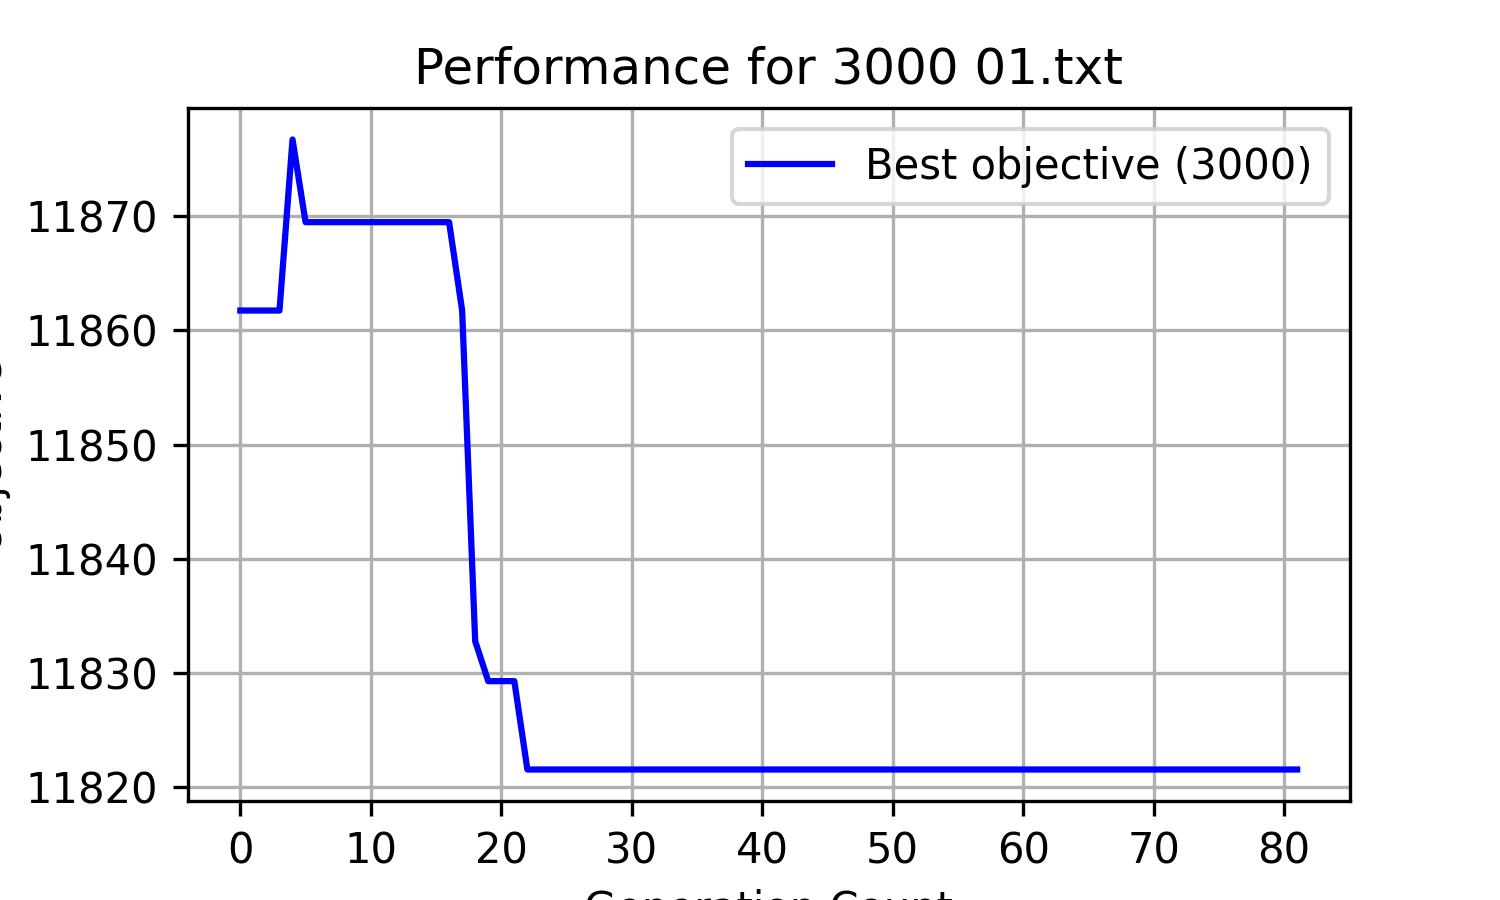
\includegraphics[width=\linewidth]{../results/5/plots/objective_vs_gen_3000_01.txt.jpg}
        \caption{Test Instance 3000 (n° 1)}
    \end{subfigure}
    \hfill
    \begin{subfigure}{0.32\textwidth}
        \centering
        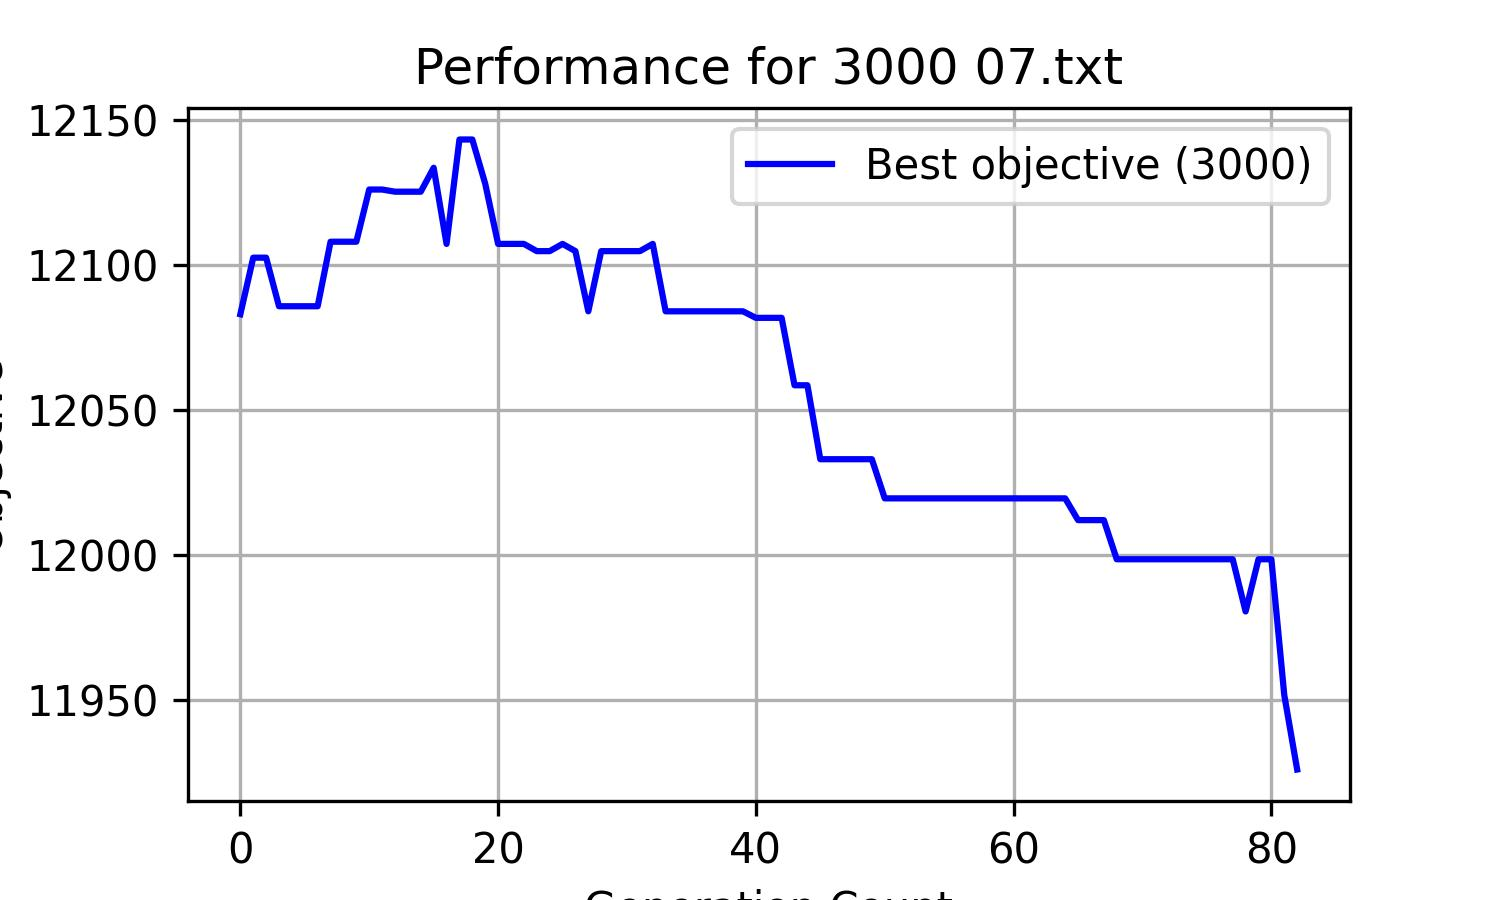
\includegraphics[width=\linewidth]{../results/5/plots/objective_vs_gen_3000_07.txt.jpg}
        \caption{Test instance 3000 (n° 7)}
    \end{subfigure}
    \hfill
    \begin{subfigure}{0.32\textwidth}
        \centering
        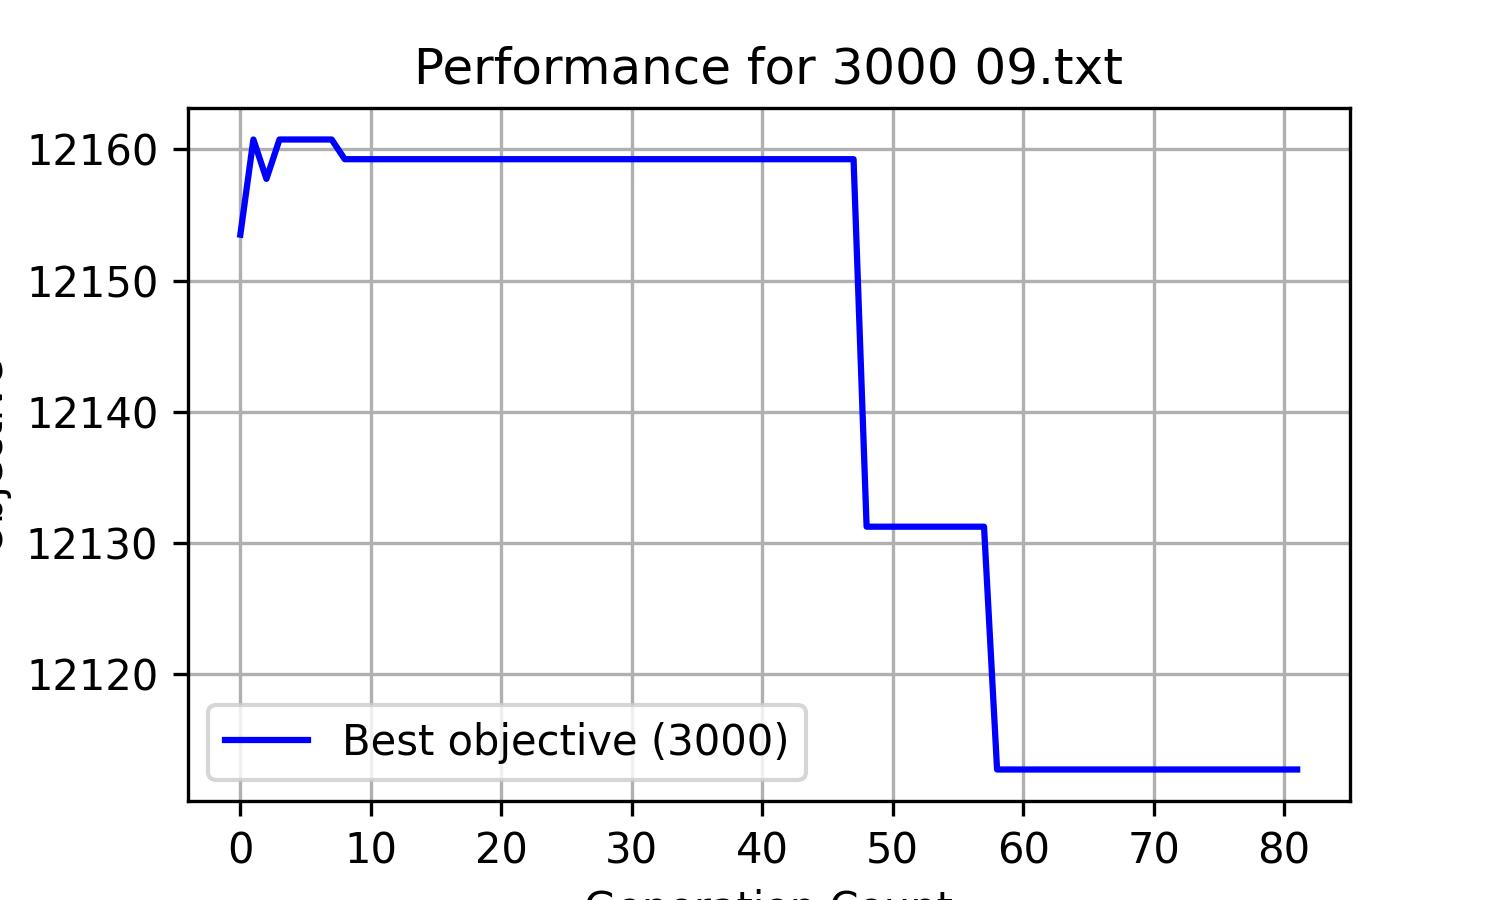
\includegraphics[width=\linewidth]{../results/5/plots/objective_vs_gen_3000_09.txt.jpg}
        \caption{Test instance 3000 (n° 9)}
    \end{subfigure}

    \caption{Objective function value by generation for different test instances}
    \label{fig:performance_plots_it5}
\end{figure}
\FloatBarrier

The remaining option is to dynamically set the number of generations depending on a dynamic convergence criteria. The chosen criteria is to stop the genetic algorithm when the average objective function value doesn't improve for 40 generations.

There could be better criteria, but this one was chosen for its simplicity. This still manages to half the number of generations for most test instances.

\begin{table}[h]
    \centering
    \begin{tabular}{|c c|}
        \hline
        \textbf{Parameter} & \textbf{Value} \\
        \hline
        POPULATION\_SIZE & 400 \\
        CXPB & 0.4 \\
        MUTPB & 0.25 \\
        K\_TOURNAMENT & 3 \\
        NUMBER\_OF\_GENERATIONS & \textbf{dynamic} \\
        \hline
    \end{tabular}
    \caption{Parameters for Iteration 5}
    \label{tab:iteration1_parameters}
\end{table}

The final results are as follows.

\begin{table}[h]
    \centering
    \begin{tabular}{|l l r r|}
        \hline
        \textbf{Problem Class} & \textbf{Test Instance} & \textbf{Average Objective} & \textbf{Average Evaluations} \\
        \hline
        LPI	& 10000	& 47784.5	& 10501.7 \\
        MPI	& 3000	& 12054.5	& 12279.1 \\
        MPI	& 2000	& 6091.0	& 12021.6 \\
        MPI	& 750	& 9460.2	& 16703.0 \\
        MPI	& 500	& 4768.6	& 18637.0 \\
        SPI	& 150	& 1264.0	& 10272.1 \\
        SPI	& 120	& 1038.2	& 10222.2 \\
        SPI	& 60	& 861.8     & 10430.5 \\
        \hline
    \end{tabular}
    \caption{Results for Iteration 5}
    \label{tab:gen_objective_summary}
\end{table}


